\chapter{Technical Background}

Over the course of the past decade, elliptic curve cryptography (henceforth referred to as ECC) has proven itself a mainstay in the wide world of applied Cryptology. While Isogeny based cryptography does build itself up from the same underlying mathematical concepts as ECC, it simultaneously draws from a slightly more complicated space of niche algebraic notions. Much of this chapter will be dedicated to illuminating these notions in a manner that should be digestable for those without serious background in algebraic geometry, or abstract algebra in general.

This chapter will cover the following preliminary topics: isogenies and their relevant properties, Supersingular Isogeny Diffie-Hellman and its related procotols, the Fiat-Shamir construction and its quantum-safe adaptation, and finally the current landscape of isogeny based signature schemes.

Our discussion of Isogenies will begin with some basic coverage of the underlying algebra. We will provide the material necessary for the remaining sections as we build up in the level of abstraction; working our way through finite fields, elliptic curves, and finally isogenies and their properties.

Once we have presented the necessary algebra, we will illustrate the specifics of the supersingular isogeny Diffie-Hellman key-exchange protocol. We will spend most of this time dedicated to a modular deconstruction of the protocol, laying bare the underlying isogeny-level procedures and algorithms which will be necessary for understanding in detail the signature protocol to come. Another task of this section will be to introduce the SIDH C library released by Microsoft Research, on top of which the core contributions of this thesis are implemented. This subsection will end with a thorough briefing and analysis of the closely related zero-knowledge proof of identity (ZKPoI) isogeny protocol proposed in the original JDP paper, as it is necessary for understanding the isogeny based signature scheme presented by Yoo et. Al.

In section 2.3 we will discuss the Fiat-Shamir transformation; a technique which, given a secure interactive proof of knowledge (/proof of identity), creates a secure digital signature scheme. We will also look at the quantum-secure adaptation published by Unruh, (applying a non-quantum-resistant transform to a quantum-resistant primitive would be rather frivolous,) 

Finally, the last section of this chapter will be dedicated to covering current isogeny-based signature schemes - the topic of which this dissertation is mainly concerned. We will primarily discuss the signature scheme of Yoo et. Al, which is a near direct application of Unruh's Fiat-Shamir adaptation to the SIDH zero-knowledge proof of identity to be discussed at the end of section 2.2.\\

\section{Algebraic Geometry \& Isogenies}
\emph{Groups \& Varieties}. A \textbf{group} is a 2-tuple composed of a set of elements and a corresponding group operation. Given some group defined by the set $G$ and the group operation $\cdot$ (written as $(G,\cdot)$) it is typical to refer to the group simply as "$G$". If $\cdot$ is equivalent to some rational mapping[footnote about rational mappings] $f_G: G \rightarrow G$, then the group $(G,\cdot)$ is said to form an \textit{algebraic variety}[footnote about the inverse function]. A group which is also an algebraic variety is referred to as an \textbf{algebraic group}.

$G$ is said to be an \emph{abelian} group if, in addition to the four traditional group axioms (closure, associativity, existence of an identity, existence of an inverse), $G$ satisfies the condition of commutitiviy. More formally, for some group $G$ with group operation $\cdot$, we say $G$ is an abelian group iff $x \cdot y = y \cdot x$ $\forall x, y \in G$. An algebraic group which is also abelian is referred to as an \textbf{abelian variety}.

\begin{definition}[Abelian Variety]
\label{defn:abelianvariety}
for some algebraic group $G$ with operation $\cdot$, we say $G$ is an \underline{abelian variety} iff $x \cdot y = y \cdot x$ $\forall x, y \in G$. 
\end{definition}

For some group $(G,\cdot)$, some $x,y \in G$, and some rational mapping $f_G: G \rightarrow G$, let the following sequence of implications denote the structure of $(G,\cdot)$:

$$
\text{group } \xRightarrow[]{x\cdot y = f_G(x,y)} \text{algebraic group } \xRightarrow[]{x\cdot y = y\cdot x} \text{abelian variety }
$$

An algebraic group $G_a$ is defined over a field $K$ if each element $e \in G_a$ is defined over $K$ and the corresponding $f_{G_a}$ is also defined over $K$. To show that a particular algebraic group $G_a$ is defined over some field $K$ we whill henceforth denote the group/field pairing as $G_a(K)$.

These algebraic structures are all important for building up to the concept of an \emph{isogeny}. The lowest-level structure we will be concerned with when discussing the forthcoming isogeny-based protocols will typically be abelian varieties. The lowest-level structure in the SIDH C codebase is a finite field element.\\\\

\noindent
\emph{Morphisms}. Let us again take for example some group $(G,\cdot)$. Let's also define some set $S_{(G,\cdot)}$ which contains every tuple $(x,y,z)$ for group elements $x,y,z$ which satisfy $x\cdot y = z$.
$$
S_{(G,\cdot)} = \{x,y,z \in G | x\cdot y = z\}
$$
Take also for example a second group $(H,*)$ and some map $\phi: G \rightarrow H$. $\phi$ is said to be \emph{structure preserving} if the following implication holds:
$$
(x,y,z) \in S_{(G,\cdot)} \Rightarrow (\phi(x),\phi(y),\phi(z)) \in S_{(H,*)}
$$

A \textbf{morphism} is simply the most general notion of a structure preserving map. More specifically, in the domain of algebraic geometry, we will be dealing with the notion of a \textbf{group homomorphism}, defined as follows:
\begin{definition}[Group Homomorphism]
\label{defn:homomorphism}
For two groups $G$ and $H$ with respective group operations $*$ and $\cdot$, a \underline{group homomorphism} is a structure preserving map $h: G \rightarrow H$ such that $\forall u, v \in G$ the following holds:
$$h(u * v) = h(u) \cdot h(v)$$
\end{definition}
From this simple definition, two more properties of homomorphisms are easily deducible. Namely, for some homomorphism $h: G \rightarrow H$, the following properties hold:
\begin{itemize}
\item $h$ maps the identity element of $G$ onto the identity element of $H$, and
\item $h(u^{-1}) = h(u)^{-1}, \forall u \in G$
\end{itemize}
Furthermore, an \textbf{endomorphism} is a special type of morphism in which the domain and the codomain are the same groups.
\begin{definition}[Endomorphism]
\label{defn:endomorphism}
For two groups $G$ and $H$, an \underline{endomorphism} is a morphism $\psi: G \rightarrow H$ wherein $G = H$
\end{definition}

\noindent
\emph{Field Extensions}.

\noindent
\emph{Quotient Groups}.

\subsection{Elliptic Curves}

An elliptic curve is an algebraic curve defineable by an equation of the form $y^2 = x^3 + ax + b$. Within algebraic geometry, it is common practice to define a group structure over elliptic curves (and any other smooth cubic curve). If we wish to define a group in accordance to a particular curve, we do so with the following notation:
$$
E: y^2 = x^3 + ax + b
$$
Wherein $E$ denotes the group in question, the elements of which are all the points (solutions) of the curve. The corresponding group operation is better understood geometrically than algebraically. Consider the following.

\begin{center}
\begin{tikzpicture}
  \draw[very thin,color=gray] (-1.9,-3.9) grid (3.9,3.9);
  \draw[->] (-2,0) -- (4.2,0) node[right] {$x$};
  \draw[->] (0,-4.2) -- (0,4.2) node[above] {$y$};
  \draw plot[id=curve, raw gnuplot, smooth] function{
    f(x,y) = y**2 - x**3 + x;
    set xrange [-4:4];
    set yrange [-4:4];
    set view 0,0;
    set isosample 1000,1000;
    set table;
    set size square;
    set cont base;
    set cntrparam levels incre 0,0.1,0;
    unset surface;
    splot f(x,y)
  };
\end{tikzpicture}
\end{center}

%\begin{figure}[htb]
%\centering
%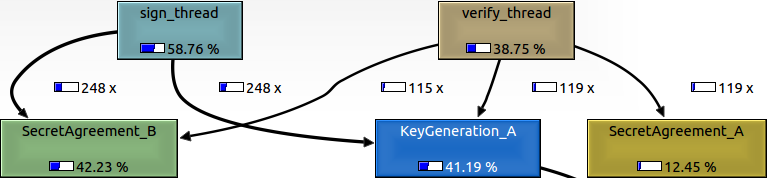
\includegraphics[scale=0.3]{signandverifycall.png} % e.g. insert ./image for image.png in the working directory, adjust scale as necessary
%\caption{Temporary. To be replaced with illustration of EC group operation.}
%\label{fig:label} % insert suitable label, this is used to refer to a fig from within the text as shown above
%\end{figure}
And so our group consists of $(E,+)$. This group operation is referred to as \emph{pointwise addition}. Additionally, we shorthand $n$-many applications of the group operation of a point $P$ to itself as $nP$, analogous to scalar multiplication. 

Moreover, groups defined over elliptic curves in this fashion constitute abelian varieties[ref]. We will see later other possible algebraic representations of elliptic curves which have varying benefits.
The point at infinity.

When referring to curves as abelian varieties defined over a field, we will write them as $E_{\alpha}(K)$, for some $\alpha$ instance of a curve and some field $K$. If we are only concerned with the geometric properties of the curve, or curves as distinct elements of some group structure, it will suffice to write $E_{\alpha}$. Moving forward from here, we will assume all general curves discussed are defined over some finite field $\mathbb{F}_q$\\

\noindent
\emph{Torsion Groups}. The $r$-\emph{torsion group} of $E$ is the set of all points $P \in E(\overline{\mathbb{F}}_q)$ such that $[r]P = \mathcal{O}$. We denote the $r$-torsion group of some curve as $E[r]$.

\noindent
\emph{Supersingular Curves}. An elliptic curve can be either \emph{ordinary} or \emph{supersingular}. There are several equivalent ways to define supersingular curves (and thus the distinction between them and ordinary curves,)

For the remainder of this paper, unless otherwise noted, all elliptic curves in discussion will be of the supersingular variety.

\subsection{Isogenies \& Their Properties}

\begin{definition}[Isogeny]
\label{defn:isogeny}
Let $G$ and $H$ be algebraic groups[ref]. An \underline{isogeny} is a morphism[ref] $h: G \rightarrow H$ possessing a finite kernel.
\end{definition}
In the case of the above definition where $G$ and $H$ are abelian varieties (such as elliptic curves,) the isogeny $h$ is homomorphic[ref] between $G$ and $H$. Because of this, isogenies over elliptic curves (and other abelian varieties) inherit certain characteristics.\\
For an isogeny $h: E_{1} \rightarrow E_{2}$ defined over elliptic curves $E_1$ and $E_2$, the following holds:
\begin{itemize}
\item $h(\mathcal{O}) = \mathcal{O}$, and
\item $h(u^{-1}) = h(u)^{-1}, \forall u \in G$
\end{itemize}

\section{Supersingular Isogeny Diffie-Hellman}

This section will aim to accomplish two things. First, we will briefly explain the isogeny-level \& key-exchange-level procedures of the SIDH protocol. Second, we will illuminate how these procedures map onto Microsoft Research's C implementation of SIDH. In this regard, this section can be considered an attempt to meld two domains of SIDH functions \& procedures, in hopes of easing the navigation from the SIDH protocol to Microsoft's C implementation, and vice versa.

The original work of De Feo, Jao, and Plut outlines three different isogeny-based cryptographic primitives: Diffie-Hellman-esque key exchange, public key encryption, and the aforementioned zero-knowledge proof of identity. Because all three of these protocols require the same initialization and public parameters, we will begin by covering these parameters in detail. Immediately after, we will analyze the key exchange at a relatively high level. Our goal of this section is to explain in detail the algorithmic and cryptographic aspects of the ZKPoI scheme, as this forms the conceptual basis for the signature scheme we will be investigating. We begin with the key exchange protocol because its sub-routines are integral to the Yoo et. Al signature implementation.

\subsection{Public Parameters}

As the name suggests, SIDH protocols work over supersingular curves (of a smooth order). Let $\mathbb{F}_q = \mathbb{F}_{p^2}$ be the finite field over which our curves are defined, $\mathbb{F}_{p^2}$ denoting the quadratic extension field of $\mathbb{F}_{p}$.  $p$ is a prime defined as follows:
$$
p = \ell_{A}^{e_A}\ell_{B}^{e_B} \cdot f \pm 1
$$
Wherein $\ell_{A}$ and $\ell_{B}$ are small primes (typically 2 \& 3, respectively) and $f$ is a cofactor ensuring the primality of $p$. We then define a global parameter curve $E$ with cardinality $(\ell_{A}^{e_A}\ell_{B}^{e_B}f)^2$.

\subsection{SIDH Key Exchange}

\subsection{Modular Breakdown}

Figure [ref] illustrates the relationship between abstraction levels of the SIDH protocol and modules of the SIDH C library.

\begin{figure}[htb]
\centering
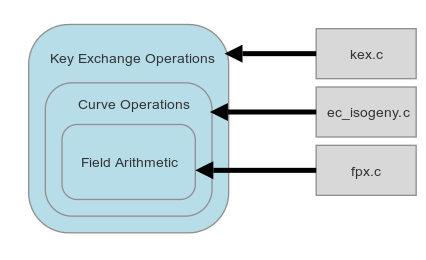
\includegraphics[scale=0.7]{halfmapwcurve.png} % e.g. insert ./image for image.png in the working directory, adjust scale as necessary
\caption{Relationship between SIDH key exchange \& MR SIDH C library}
\label{fig:halfmap} % insert suitable label, this is used to refer to a fig from within the text as shown above
\end{figure}


\subsection{Security Assumptions}



\subsection{Zero-Knowledge Proof of Identity}

Recall the notion of a simple identification scheme:

\section{Fiat-Shamir Construction}

The Fiat-Shamir construction (sometimes referred to as the Fiat-Shamir heuristic or transform) is used

\subsection{Unruh's Post-Quantum Adaptation}



\section{Isogeny Based Signatures}

Now that we've introduced the zero-knowledge proof of identity scheme from [REFERENCE] as well as Unruh's quantum-safe Fiat-Shamir adaption, the isogeny based signature scheme presented by Yoo et. Al is a near-trivial application of the latter to the former. 

The isogeny based signature scheme presented by Yoo et. Al is defined, in the traditional manner, by a tuple of algorithms. Namely, the scheme is defined by the tuple (KeyGen, Sign, Verify) with each algorithm loosely defined as follows:\\
\textbf{KeyGen(}\textbf{)}: Select a random point $S$ of order $\ell_{A}^{e_A}$, compute the isogeny $\phi: E \rightarrow E/ \langle S \rangle$. Return (pk, sk) where pk = $(E/ \langle S \rangle, \phi(P_B), \phi(Q_B))$ and sk = $S$.\\
\textbf{Sign()}:\\
\textbf{Verify()}:\\


\subsection{Modular Breakdown}

\begin{figure}[htb]
\centering
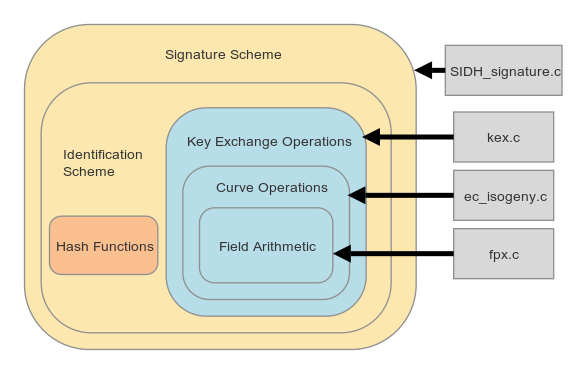
\includegraphics[scale=0.7]{fullmapwcurve.png} % e.g. insert ./image for image.png in the working directory, adjust scale as necessary
\caption{Relationship between SIDH key exchange \& MR SIDH C library}
\label{fig:halfmap} % insert suitable label, this is used to refer to a fig from within the text as shown above
\end{figure}


Shortly after, the following, more in-depth algorithms are given as definitions: 

\begin{algorithm}
\caption{KeyGen($\lambda$)}\label{euclid}
\begin{algorithmic}[1]
\State Pick a random point S of order $\ell^{e_{A}}_{A}$
\State Compute the isogeny $\phi: E \rightarrow E/\langle S \rangle$
\State pk $\gets (E/\langle S \rangle, \phi(P_{B}), \phi(Q_{B}))$
\State sk $\gets S$
\State \Return (pk,sk)
\end{algorithmic}
\end{algorithm}

\begin{algorithm}
\caption{Sign(sk, $m$)}\label{euclid}
\begin{algorithmic}[1]
\For{\texttt{i = 1..2$\lambda$}}
	\State Pick a random point R of order $\ell^{e_{B}}_{B}$
	\State Compute the isogeny $\psi: E \rightarrow E/\langle R \rangle$
	\State Compute either $\phi' : E/\langle R \rangle \rightarrow E/\langle R,S \rangle$ or $\psi' : E/\langle S \rangle \rightarrow E/\langle R,S \rangle$
	\State $(E_{1},E_{2}) \gets (E/\langle R \rangle, E/\langle R,S \rangle)$
	\State $\texttt{com}_{i} \gets (E_{1}, E_{2})$
	\State $\texttt{ch}_{i,0} \gets_{R} \{0,1\}$
	\State $(\texttt{resp}_{i,0}, \texttt{resp}_{i,1}) \gets ((R,\phi(R)), \psi(S))$
	\If{$\texttt{ch}_{i,0} = 1$}
		\State $\texttt{swap}(\texttt{resp}_{i,0},\texttt{resp}_{i,1})$
	\EndIf
	\State $h_{i,j} \gets G(\texttt{resp}_{i,j})$
\EndFor

\State $J_{1} \parallel ... \parallel J_{2\lambda} \gets H(pk, m, (\texttt{com}_{i})_{i},(\texttt{ch}_{i,j})_{i,j},(h_{i,j})_{i,j})$

\State \Return $\sigma \gets ((\texttt{com}_{i})_{i}, (\texttt{ch}_{i,j})_{i,j}, (h_{i,j})_{i,j}, (\texttt{resp}_{i,J_{i}})_{i})$
\end{algorithmic}
\end{algorithm}

\begin{algorithm}[H]
\caption{Verify(pk, $m$, $\sigma$)}\label{euclid}
\begin{algorithmic}[1]
\State $J_{1} \parallel ... \parallel J_{2\lambda} \gets H(pk, m, (\texttt{com}_{i})_{i},(\texttt{ch}_{i,j})_{i,j},(h_{i,j})_{i,j})$
\For{\texttt{i = 0..2$\lambda$}}
	\State \textbf{check} $h_{i,J_{i}} = G(\texttt{resp}_{i,J_{i}})$
	\If{$\texttt{ch}_{i,J_{i}} = 0$}
		\State Parse $(R,\phi(R)) \gets \texttt{resp}_{i,J_{i}}$
		\State \textbf{check} $(R, \phi(R))$ have order $\ell^{e_{B}}_{B}$
		\State \textbf{check} $R$ generates the kernel of the isogeny $E \rightarrow E_{1}$
		\State \textbf{check} $\phi(R)$ generates the kernel of the isogeny $E/\langle S \rangle \rightarrow E_{2}$
	\Else
		\State Parse $\psi(S) \gets \texttt{resp}_{i,J_{i}}$
		\State \textbf{check} $\psi(S)$ has order $\ell^{e_{A}}_{A}$
		\State \textbf{check} $\psi(S)$ generates the kernel of the isogeny $E_{1} \rightarrow E_{2}$
	\EndIf
\EndFor

\If{all checks succeed}
	\State \Return 1
\EndIf
\end{algorithmic}
\end{algorithm}

If we transcribe the above to the language of the Microsoft SIDH API, we have in essense the following:\\

\begin{algorithm}
\caption{KeyGen($\lambda$)}\label{euclid}
\begin{algorithmic}[1]
\State (pk, sk) $\gets \texttt{KeyGeneration\_B()}$
\State \Return (pk,sk)
\end{algorithmic}
\end{algorithm}

\begin{algorithm}
\caption{Sign(sk, $m$)}\label{euclid}
\begin{algorithmic}[1]
\For{\texttt{i = 1..2$\lambda$}}
	\State $(, R, \psi) \gets \texttt{KeyGeneration\_A(E)}$
	\State $E_{1} \gets E/\langle R \rangle$
	\State $(E_{2},E/\langle R,S \rangle) \gets \texttt{SecretAgreement\_B()}$
	\State $(E_{1},E_{2}) \gets (E/\langle R \rangle, E/\langle R,S \rangle)$
	\State $\texttt{com}[i] \gets (E_{1}, E_{2})$
	\State $\texttt{ch}[i] \gets_{R} \{0,1\}$
	\State $(\texttt{resp}[i]_{0}, \texttt{resp}[i]_{1}) \gets ((R,\phi(R)), \psi(S))$
	
%% this portion was skipped?	
%%	\If{$\texttt{ch}[i] = 1$}
%%		\State $\texttt{swap}(\texttt{resp}[i]_{0},\texttt{resp}[i]_{1})$
%%	\EndIf
%%	\State $h_{i,j} \gets G(\texttt{resp}[i]_{j})$
\EndFor

\State $J_{1} \parallel ... \parallel J_{2\lambda} \gets H(pk, m, (\texttt{com}_{i})_{i},(\texttt{ch}_{i})_{i},(h_{i,j})_{i,j})$

\State \Return $\sigma \gets ((\texttt{com}_{i})_{i}, (\texttt{ch}_{i,j})_{i,j}, (h_{i,j})_{i,j}, ((\texttt{resp})[J_{i}])$
\end{algorithmic}
\end{algorithm}
